%iffalse
\let\negmedspace\undefined
\let\negthickspace\undefined
\documentclass[journal,12pt,onecolumn]{IEEEtran}
\usepackage{cite}
\usepackage{amsmath,amssymb,amsfonts,amsthm}
\usepackage{algorithmic}
\usepackage{graphicx}
\usepackage{textcomp}
\usepackage{xcolor}
\usepackage{txfonts}
\usepackage{listings}
\usepackage{enumitem}
\usepackage{mathtools}
\usepackage{gensymb}
\usepackage{comment}
\usepackage[breaklinks=true]{hyperref}
\usepackage{tkz-euclide} 
\usepackage{gvv}                                        
%\def\inputGnumericTable{}                                 
\usepackage[latin1]{inputenc}     
\usepackage{xparse}
\usepackage{color}                                            
\usepackage{array}                                            
\usepackage{longtable}                                       
\usepackage{calc}                                             
\usepackage{multirow}
\usepackage{multicol}
\usepackage{hhline}                                           
\usepackage{ifthen}                                           
\usepackage{lscape}
\usepackage{tabularx}
\usepackage{array}
\usepackage{float}
\newtheorem{theorem}{Theorem}[section]
\newtheorem{problem}{Problem}
\newtheorem{proposition}{Proposition}[section]
\newtheorem{lemma}{Lemma}[section]
\newtheorem{corollary}[theorem]{Corollary}
\newtheorem{example}{Example}[section]
\newtheorem{definition}[problem]{Definition}
\newcommand{\BEQA}{\begin{eqnarray}}
\newcommand{\EEQA}{\end{eqnarray}}
\newcommand{\define}{\stackrel{\triangle}{=}}
\theoremstyle{remark}
\newtheorem{rem}{Remark}
% Marks the beginning of the document
\begin{document}
\title{AR:ARCHITECTURE AND PLANNING}
\large \author{AI25btech11027 - Bhuvana}
\maketitle
\renewcommand{\thefigure}{\theenumi}
\renewcommand{\thetable}{\theenumi}
\begin {center}
\large \textbf{2011}\\
{Duration:Three hours \hfill Maximum Marks:150}
\end{center}
{\textbf{Q.1 to Q.25 carry one mark each.}
\begin{enumerate}
    \item Capital town of Gandhinagar has been designed by \hfill \textbf{(GATE EE 2025)}
    \begin{enumerate}
    \begin{multicols}{4}
        \item Norman Foster
        \item B.V.Doshi
        \item H.K.Mewada
        \item Le Corbusier
        \end{multicols}
    \end{enumerate}
    \item Rajiv Awas Yojana of Ministry of Housing,Government of India addresses housing for \hfill \textbf{(GATE EE 2025)}
    \begin{enumerate}
        \begin{multicols}{2}
            \item Middle Income Group
            \item Low Income Group
            \item High Income Group
            \item Slum Dwellers
        \end{multicols}
    \end{enumerate}
    \item The triangular space formed by two consecutive arches is \hfill \textbf{(GATE EE 2025)}
    \begin{enumerate}
        \begin{multicols}{4}
            \item Tympanum
            \item Spandrel
            \item Regula
            \item Extrados
        \end{multicols}
    \end{enumerate}
\item Rose Window is an iconic feature of \hfill \textbf{(GATE EE 2025)}
\begin{enumerate}
    \begin{multicols}{2}
        \item Notre Dame,Paris
        \item Hagia Sophia,Istanbul
        \item St.Peter's ,Rome
        \item Victoria Memorial,Kolkata
    \end{multicols}
\end{enumerate}
\item Purity of colour is described by \hfill \textbf{(GATE EE 2025)}
\begin{enumerate}
    \begin{multicols}{4}
        \item Hue
        \item Value
        \item Chroma
        \item Tone
    \end{multicols}
\end{enumerate}
\item A slab simply supported on all its edges with a ratio of longer side to shorter side greater or equal to $2.0$ is designed as \hfill \textbf{(GATE EE 2025)}
\begin{enumerate}
    \begin{multicols}{2}
        \item One way slab
        \item Two way slab
        \item Flat slab
        \item Coffered slab
    \end{multicols}
\end{enumerate}
\item Entablature consists of \hfill \textbf{(GATE EE 2025)}
\begin{enumerate}
    \begin{multicols}{2}
        \item Architrave,Tenia,Cornice
        \item Architrave,Frieze,Cornice
        \item Frieze,Cornice,Triglyphs
        \item Cornice,Guttae,Tympanum
    \end{multicols}
\end{enumerate}
\item Town planned for \texttt{Motor Age} refers to \hfill \textbf{(GATE EE 2025)}
\begin{enumerate}
    \begin{multicols}{2}
        \item Toronto,Ontario
        \item Nassan Shores,Long Island
        \item Radburn,New Jersey
        \item Green Belt,Maryland
    \end{multicols}
\end{enumerate}
\item The minimum road curb length required for parking $10$ cars perpendicular to the road is \hfill \textbf{(GATE EE 2025)}
\begin{enumerate}
    \begin{multicols}{2}
        \item $15$ m
        \item $25$ m
        \item $35$ m
        \item $40$ m
    \end{multicols}
\end{enumerate}
\item Which of the following generates heat island? \hfill \textbf{(GATE EE 2025)}
\begin{enumerate}
    \begin{multicols}{2}
        \item Urban areas
        \item Coastal areas
        \item Wetlands
        \item Forest areas
    \end{multicols}
\end{enumerate}
\item The most suitable earthquake resistant built plan form is \hfill \textbf{(GATE EE 2025)}
\begin{figure}[H]
    \centering
    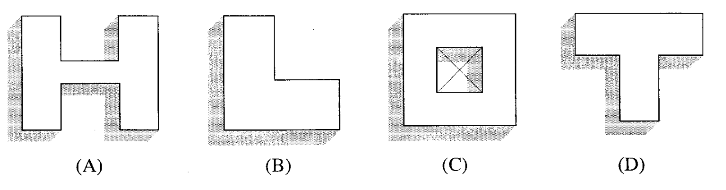
\includegraphics[width=0.5\linewidth]{figs/fig1.png}
    \caption{}
    \label{fig1}
\end{figure}
\item Transfer of Development Right (TDR) is a tool used for \hfill \textbf{(GATE EE 2025)}
\begin{enumerate}
    \begin{multicols}{2}
        \item Human development
        \item Land development
        \item Economic development
        \item Infrastructure development
    \end{multicols}
\end{enumerate}
\item Dandaka form of settlement layout is basically a \hfill \textbf{(GATE EE 2025)}
\begin{enumerate}
    \begin{multicols}{2}
        \item Grid Iron pattern
        \item Ring radical pattern
        \item Radical pattern
        \item Informal pattern
    \end{multicols}
\end{enumerate}
\item Maximum horizontal angle from the speaker in a seating area of a lecture theatre should be \hfill \textbf{(GATE EE 2025)}
\begin{enumerate}
    \begin{multicols}{4}
        \item $70^\circ$
        \item $90^\circ$
        \item $120^\circ$
        \item $140^\circ$
    \end{multicols}
\end{enumerate}
\item \texttt{U-value} refers to \hfill \textbf{(GATE EE 2025)}
\begin{enumerate}
    \item Utility function for convective heat transfer
    \item Thermal transmittance of building components
    \item Energy transfer between thermal bridges
    \item Measure for area related heating and cooling loads
\end{enumerate}
\item Consistency of cement is measured by \hfill \textbf{(GATE EE 2025)}
\begin{enumerate}
    \begin{multicols}{2}
        \item Pycometer
        \item Slump cone
        \item Universal Testing Machine
        \item Vicat's apparatus
    \end{multicols}
\end{enumerate}
\item The appropriate material for flooring of an external ramp of a building would be \hfill \textbf{(GATE EE 2025)}
\begin{enumerate}
    \begin{multicols}{2}
        \item Polished granite
        \item Wax polished marble
        \item Glazed ceramic tile
        \item Rough finish sandstone
    \end{multicols}
\end{enumerate}
\item Which of the following is \textbf{NOT} a member of a steel Truss? \hfill \textbf{(GATE EE 2025)}
\begin{enumerate}
    \begin{multicols}{4}
        \item Gusset plate
        \item Wall plate
        \item Fish plate
        \item Anchor Bolts
    \end{multicols}
\end{enumerate}
\item Identify the odd among the following \hfill \textbf{(GATE EE 2025)}
\begin{enumerate}
    \begin{multicols}{2}
        \item Security deposit
        \item Professional tax
        \item Performance bank guarantee
        \item Earnest money
    \end{multicols}
\end{enumerate}
\item Weep hole is a term used to describe \hfill \textbf{(GATE EE 2025)}
\begin{enumerate}
    \item Perforations in the cast iron pipe used for bording
    \item Holes in retaining wall for draining water
    \item Holes in the cover plate of floor traps
    \item Holes dug in earth to recharge ground water
\end{enumerate}
\item Busway,Busduct and Raceway are components of \hfill \textbf{(GATE EE 2025)}
\begin{enumerate}
    \begin{multicols}{2}
        \item Security system
        \item Air conditioning system
        \item Eletrical system
        \item Water supply system
    \end{multicols}
\end{enumerate}
\item The difference between Wet Bulb Temparature and Dry Bulb Temparature is called \hfill \textbf{(GATE EE 2025)}
\begin{enumerate}
    \begin{multicols}{2}
        \item Dry bulb depression
        \item Wet bulb depression
        \item Variable depression
        \item Atmospheric depression    \end{multicols}
\end{enumerate}
\item In India, one of the Slum Implrovement initiatives is \hfill \textbf{(GATE EE 2025)}
\begin{enumerate}
    \begin{multicols}{2}
        \item Special Residentia Zone
        \item Valmiki Ambedkar Malin Basti Awas Yojana
        \item Indira Awas Yojana
        \item Eco Housing
    \end{multicols}
\end{enumerate}
\item Suspended Floors is a structural system used in \hfill \textbf{(GATE EE 2025)}
\begin{enumerate}
    \begin{multicols}{2}
        \item Lloyds Building,London
        \item Jin Mao Building,Shanghai
        \item Petronas Tower,Kualalampur
        \item Hongkong Shanghai Bank,Hongkong
    \end{multicols}
\end{enumerate}
\item Residual method of valuation is used to determine \hfill \textbf{(GATE EE 2025)}
\begin{enumerate}
    \begin{multicols}{2}
        \item Public Private Partnership Deal
        \item Rent
        \item Property Tax
        \item Selling Price
    \end{multicols}
\end{enumerate}
\textbf{Q.26 to Q.55 carry two marks each.}
\item Match the buildings in \textbf{Group I} with their architect in \textbf{Group II} \hfill \textbf{(GATE EE 2025)}
\\
\begin{tabular}{p{0.4\textwidth}p{0.5\textwidth}}
 \textbf{Group I}    & \textbf{Group II} \\
P. Bibliotheca Alexandrina,Alexandria     & 1. I.M.Pei\\
Q. Institut du Monde Arab,Paris & 2. Jean Nouvel\\
R. Bank of China,Hongkong & 3. Daniel Libeskind\\
S. Jewish Museum,Berlin & 4. Renzo Piano\\
  & 5. Sn\o hetta
\end{tabular}
\begin{enumerate}
    \begin{multicols}{2}
        \item P-5,Q-2,R-1,S-4
        \item P-5,Q-4,R-1,S-3
        \item P-4,Q-2,R-5,S-3
        \item P-5,Q-2,R-1,S-3
    \end{multicols}
\end{enumerate}
\item A room measuring $5$ m $*$ $3.5$ m enclosed by brick wall has a ceiling at $3$ m height. The room has a door and a window opening of $1$ m $*$ $2$ m and $1$ m $*$ $1$ m respectively.The quantity of plastering required for interior walls (in sqm) is \hfill \textbf{(GATE EE 2025)}
\begin{enumerate}
    \begin{multicols}{4}
        \item $46.5$
        \item $48$
        \item $51$
        \item $68.5$
    \end{multicols}
\end{enumerate}
\item One cubic metre of Ordinary Portland Cement yeilds a volume of M15 concrete in the range of \hfill \textbf{(GATE EE 2025)}
\begin{enumerate}
    \begin{multicols}{4}
        \item $2$ to $3$ cum
        \item $4$ to $5$ cum
        \item $7$ to $8$ cum
        \item $8$ to $9$ cum
    \end{multicols}
\end{enumerate}
\item Match the CAD commands in \textbf{Group I} with their functions in \textbf{Group II} \hfill \textbf{(GATE EE 2025)}
\\
\begin{tabular}{p{0.4\textwidth}p{0.5\textwidth}}
\textbf{Group I}     & \textbf{Group II} \\
 P. LAYISO    & 1. blends selected object to destination layer\\
 Q. LAYMCH  & 2. freezes layer of selected object\\
 R. LAYMRG  & 3. hides or locks layers other than those of selected objects\\
 S. LAYLCK  & 4. assign selected object to destination layer\\
       & 5. locks object of destination layer\\
\end{tabular}
\begin{enumerate}
    \begin{multicols}{2}
        \item P-2,Q-4,R-1,S-5
        \item P-3,Q-2,R-1,S-5
        \item P-3,Q-5,R-4,S-2
        \item P-3,Q-4,R-1,S-5
    \end{multicols}
\end{enumerate}
\item Match the buildings in \textbf{Group I} with their corresponding structual forms in \textbf{Group II}. \hfill \textbf{(GATE EE 2025)}
\\
\begin{tabular}{p{0.4\textwidth}p{0.5\textwidth}}
\textbf{Group I}     & \textbf{Group II}  \\
P. Hall of Nations,New Delhi     & 1. Spherical Structure\\
Q. Salvacao Church,Mumbai  & 2. Folded Plates\\
R. State Trading Corporation Building,New Delhi & 3. Octahedral lattice structure\\
S. Matrimandir,Auroville & 4. Vierendeel girders\\
   & 5. Shell roof structue\\
\end{tabular}
\begin{enumerate}
    \begin{multicols}{2}
        \item P-3,Q-5,R-4,S-1
        \item P-2,Q-5,R-4,S-1
        \item P-3,Q-5,R-4,S-2
        \item P-3,Q-5,R-2,S-1
    \end{multicols}
\end{enumerate}
\item Identify the \textbf{INCORRECT} statements \hfill \textbf{(GATE EE 2025)}
\begin{enumerate} 
    \item Guggenheim,Bilbao is an example of Deconstructivism.
    \item Silver Abstraction is a term used metal clad modern high rise buildings
    \item Spiral Building in Tokyo has a curvilinear built form.
    \item Free Building plan form is a concept given by Le Corbusier
\end{enumerate}
\item Match the terms in \textbf{Group I} with their features in \textbf{Group II} \hfill \textbf{(GATE EE 2025)}
\\
\begin{tabular}{p{0.4\textwidth}p{0.5\textwidth}}
\textbf{Group I}     & \textbf{Group II}  \\
 P. Quoin   & 1. Geometric representation of the universe\\
 Q. Stucco  & 2. Small dome\\
 R. Mandala & 3. Triangular form above an opening\\
 S. Cupola  & 4. Corner stone at the angle of buildings\\
\end{tabular}
\begin{enumerate}
    \begin{multicols}{2}
        \item P-4,Q-3,R-2,S-1
        \item P-3,Q-5,R-1,S-4
        \item P-4,Q-5,R-1,S-2
        \item P-3,Q-1,R-5,S-2
    \end{multicols}
\end{enumerate}
\item Match the architectural styles in \textbf{Group I} with their features in \textbf{Group II}. \hfill \textbf{(GATE EE 2025)}
\\
\begin{tabular}{p{0.4\textwidth}p{0.5\textwidth}}
 \textbf{Group I}    &\textbf{Group II}  \\
P. West Asiatic     & 1. Arches and pendentives\\
Q. Greek & 2. Small dome\\
R. Mandala & 3. Triangular form above an opening\\
S. Cupola & 4. Corner stone at the angle of buildings\\
      & 5. Plaster\\
\end{tabular}
\begin{enumerate}
    \begin{multicols}{2}
        \item P-3,Q-2,R-1,S-4
        \item P-5,Q-4,R-1,S-2
        \item P-5,Q-4,R-1,S-3
        \item P-4,Q-3,R-5,S-2
    \end{multicols}
\end{enumerate}
\item Gestalt's Laws of visual perception \textbf{DO NOT} relate to \hfill \textbf{(GATE EE 2025)}
\begin{enumerate}
    \item Aesthetic of form are a function of Golden Section
    \item Things are perceived as a whole
    \item Whole thing is greater than the sum total of its parts
    \item Elements with continuity are perceived together
\end{enumerate}
\item A site in a map drawn to scale of $1:16000$ measures $75$ sqcm. The actual area of the site in hectares is \hfill \textbf{(GATE EE 2025)}
\begin{enumerate}
    \begin{multicols}{2}
        \item $120$
        \item $162$
        \item $192$
        \item $256$
    \end{multicols}
\end{enumerate}
\item Identify the \textbf{CORRECT} CAD statements \hfill \textbf{(GATE EE 2025)}
\\
P. SPLINE connects sequence of line segments into a single object
\\
Q. SPLINE is a smooth curve passing through or near a given set of points
\\
R. PLINE creates straight line segments,arc segments or both
\\
S. PLINE can be closed only when its start and end points are coincident and tangent
\\
T. PLINE allows adjusting the width and curvature of its multiline segments
\\
U. SPLINE can be explored into smaller segments
\\
V. PLINE can be converted into a continuous curve segment
\begin{enumerate}
    \begin{multicols}{4}
        \item P,R,S,U
        \item Q,R,T,V
        \item R,S,T,V
        \item S,T,U,V
    \end{multicols}
\end{enumerate}
\item Match the eminent personalities in \textbf{Group I} with their books and statements in \textbf{Group II} \hfill \textbf{(GATE EE 2025)}
\\
\begin{tabular}{p{0.4\textwidth}p{0.5\textwidth}}
\textbf{Group I}     & \textbf{Group II} \\
P. Kevin Lynch     & 1. The Fountainhead\\
Q. Ayn Rand & 2. Small is Beautiful\\
R. Paul D.Spreiregen & 3. Site Planning\\
S. E.F.Schumacher & 4. Urban Design:Architecture of Towns and Cities\\
       & 5. Design of Cities\\
\end{tabular}
\begin{enumerate}
    \begin{multicols}{2}
        \item P-4,Q-2,R-5,S-3
        \item P-3,Q-1,R-2,S-5
        \item P-5,Q-1,R-4,S-2
        \item P-3,Q-1,R-4,S-2
    \end{multicols}
\end{enumerate}
\item Match the urbans forms listed in \textbf{Group I} with the towns listed in \textbf{Group II} \hfill \textbf{GATE EE 2025)}
\\
\begin{tabular}{p{0.4\textwidth}p{0.4\textwidth}}
\textbf{Group I}     & \textbf{Group II} \\
P. Grid Iron     & 1. New Delhi\\
Q. Radical   &  2. Washington D.C.\\
R. Linear  & 3. Copenhagen\\
S. Finger plan & 4. Mumbai\\
           & 5. Canberra\\
\end{tabular}
\begin{enumerate}
    \begin{multicols}{2}
        \item P-2,Q-1,R-4,S-3
        \item P-3,Q-1,R-2,S-5
        \item P-3,Q-1,R-4,S-2
        \item P-2,Q-1,R-4,S-5
    \end{multicols}
\end{enumerate}
\item Consider the following features \hfill \textbf{(GATE EE 2025)}
\\
1. Length finely proportional to its width
\\
2. Statues as silhouettes against the sky above cornice lines 
\\
3. Fountains significantly fine vintage points
\\
4. Series of different shapes connected by traditional narrow streets,column screens or arches 
\\
The element of urban design which comprises the above is
\begin{enumerate}
    \begin{multicols}{2}
        \item Vista
        \item Piazza
        \item Rond Point
        \item Bosque
    \end{multicols}
\end{enumerate}
\item Match the instruments in \textbf{Group I} with their corresponding functions in \textbf{Group II} \hfill \textbf{(GATE EE 2025)}
\\
\begin{tabular}{p{0.45\textwidth}p{0.45\textwidth}}
\textbf{Group I} & \textbf{Group II}\\
P. Hygrometer & 1. Precipitation  \\
Q. Disdrometer  & 2. Vapor Pressure\\
R. Anemometer  & 3. Solar Radiation\\
S. Manometer  & 4. Relative Humidity\\
              & 5. Velocity of Air\\
\end{tabular}
\begin{enumerate}
    \begin{multicols}{2}
        \item P-4,Q-1,R-2,S-3
        \item P-4,Q-3,R-2,S-5
        \item P-1,Q-2,R-5,S-4
        \item P-4,Q-1,R-5,S-2
    \end{multicols}
\end{enumerate}
\item Match the instuments in \textbf{Group I} with their corresponding functions in \textbf{Group II} \hfill \textbf{(GATE EE 2025)}
\\
\begin{tabular}{p{0.6\textwidth}p{0.4\textwidth}}
\textbf{Group I}     &\textbf{Group II}  \\
P. Symmetrical layout,water cascades,entombment     & 1. French gardens\\
Q. Radical layout,symmetrical sculptures,boulevards & 2. English gardens\\
R. Occult symmetry,pontoon bridges,stepping stones & 3. Chinese gardens\\
S. Hierarchy of courts,hierarchy of gates,zoomorphic forms & 4. Mughal gardens\\
   & 5. Japanese gardens\\
\end{tabular}
\begin{enumerate}
    \begin{multicols}{2}
        \item P-2,Q-1,R-4,S-3
        \item P-4,Q-1,R-5,S-3
        \item P-4,Q-3,R-5,S-1
        \item P-5,Q-1,R-2,S-3
    \end{multicols}
\end{enumerate}
\item Arrange the following sense of enclosures in a hierarchy of decreasing order \hfill \textbf{(GATE EE 2025)}
\begin{figure}[H]
    \centering
    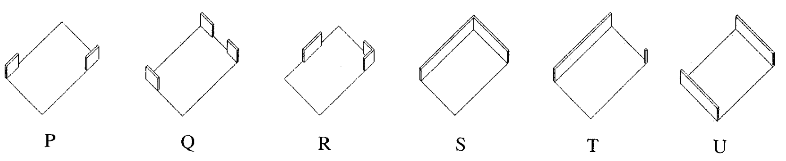
\includegraphics[width=0.5\linewidth]{figs/fig2.png}
    \caption{}
    \label{fig2}
\end{figure}
\begin{enumerate}
    \begin{multicols}{2}
        \item $S>Q>U>P>T>R$
        \item $U>S>Q>R>P>T$
        \item $P>Q>R>S>T>U$
        \item $T>P>S>Q>U>R$
    \end{multicols}
\end{enumerate}
\item Match the elements of \textbf{Group I} with their corresponding type in \textbf{Group II} \hfill \textbf{(GATE EE 2025)}
\\
\begin{tabular}{p{0.4\textwidth}p{0.4\textwidth}}
\textbf{Group I} & \textbf{Group II}\\
P. Fire hydrant     & 1. Street Furniture \\
Q. Planter beds     & 2. Street Hardware\\
R. Letter box & \\
S. Traffic signs & \\
T. Lamp Posts & \\
\end{tabular}
\begin{enumerate}
    \begin{multicols}{2}
        \item P-2,Q-1,R-1,S-2,T-2
        \item P-1,Q-1,R-2,S-1,T-1
        \item P-1,Q-1,R-2,S-2,T-2
        \item P-2,Q-1,R-2,S-2,T-2
    \end{multicols}
\end{enumerate}
\item In a construction project schedule. A is the first activity .Activities B \& C follow A. Activity D follows B \& C. Activity E follows C. Activity F follows D \& E.\hfill \textbf{(GATE EE 2025)}
\begin{table}[h]
    \centering
    \begin{tabular}{|c|c|c|c|c|c|c|} \hline
 \textbf{Activity} & A & B & C & D & E & F\\ \hline
 \textbf{Duration} & $3$ & $2$ & $5$ & $6$ & $5$ & $3$ \\ \hline   
    \end{tabular}
\end{table}
\\
The critical time to complete the project will be
\begin{enumerate}
    \begin{multicols}{4}
        \item $14$ days
        \item $16$ days
        \item $17$ days
        \item $20$ days
    \end{multicols}
\end{enumerate}
\item The maintenance cost of a building will be Rs.$2$ lakhs after 10 years. The The annual sinking fund required for such maintenance @ $6\%$ interest per annum will be \hfill \textbf{(GATE EE 2025)}
\begin{enumerate}
    \begin{multicols}{4}
        \item Rs.$17,200$/-
        \item Rs.$15,200$/-
        \item Rs.$13,200$/-
        \item Rs.$11,200$/-
    \end{multicols}
\end{enumerate}
\item  Match the figures in \textbf{Group I} with the fixtures in \textbf{Group II} \hfill \textbf{(GATE EE 2025)}
\begin{figure}
    \centering
    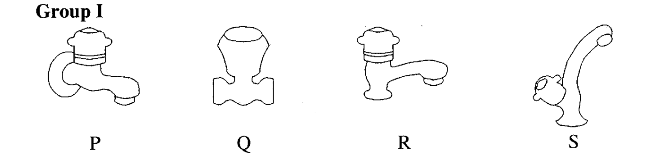
\includegraphics[width=0.5\linewidth]{figs/fig3.png}
    \caption{}
    \label{fig3}
\end{figure}
\textbf{Group II:} 
\begin{multicols}{4}
1. Sink Cock 
2. Bib Cock 
3. Pillar Cock
4. Stop Cock 
\end{multicols}

\begin{enumerate}
\begin{multicols}{2}
\item P-1, Q-4, R-2, S-3 
\item  P-2, Q-3, R-1, S-4
\item P-3, Q-1, R-2, S-4 
\item P-2, Q-4, R-3, S-1 
\end{multicols}
\end{enumerate}
\item  Match the joints in Group I with the corresponding figures in Group II \hfill \textbf{(GATE EE 2025)}
\textbf{Group I:} 
\begin{multicols}{4}
P. Butt joint 
Q. Rebated joint
R. Table joint 
S. Tongue \& Groove joint 
\end{multicols}
\begin{figure}[H]
    \centering
    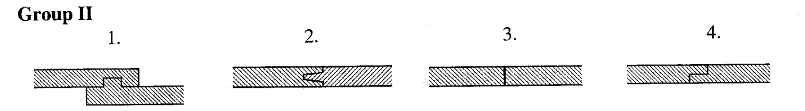
\includegraphics[width=0.5\linewidth]{figs/fig4.png}
    \caption{}
    \label{fig4}
\end{figure}
\begin{enumerate}
\begin{multicols}{2}
\item P-3, Q-4, R-1, S-2 
\item P-4, Q-1, R-3, S-2 
\item P-3, Q-1, R-2, S-4 
\item P-3, Q-4, R-2, S-1
\end{multicols}
\end{enumerate}
\textbf{Common Data Questions}

\textbf{Common Data for Questions 48 and 49:} 
A beam of span $L$ is simply supported at two ends. One half span of the beam weighs $W$ and the remaining half span weighs $2W$.

\item Maximum shear force in the beam will be:\hfill \textbf{(GATE EE 2025)}
\begin{enumerate}
\begin{multicols}{4}
\item $W$
\item $1.25W$
\item $1.75W$
\item $3W$
\end{multicols}
\end{enumerate}

\item Maximum bending moment will occur at: \hfill \textbf{(GATE EE 2025)}
\begin{enumerate}
\begin{multicols}{2}
\item $L/16$ from midpoint of the beam
\item Midpoint of the beam
\item $L/7$ from midpoint of the beam
\item One of the endpoints of the beam
\end{multicols}
\end{enumerate}

\textbf{Common Data for Questions 50 and 51:}
\\
A building site has a plot of $500 \ \text{sqm}$ 
\\
    
Maximum allowable height = $G+7$ \quad Area to be utilized for paved access roads = $10\%$ \\ 
Maximum ground coverage = $40\%$ \quad Runoff coefficient for paved surface = 0.9\\
Maximum allowable FAR = 2.0 \quad \quad Runoff coefficient for unpaved surface = 0.3\\


\item If maximum allowable FAR is utilized, the minimum ground coverage would be: \hfill \textbf{(GATE EE 2025)}
\begin{enumerate}
\begin{multicols}{4}
\item $20\%$
\item $25\%$
\item $30\%$
\item $35\%$
\end{multicols}
\end{enumerate}

\item If it rains for 30 min with an intensity of $10\ \text{cm/hr}$, minimum volume of rain water that can be collected will be: \hfill \textbf{(GATE EE 2025)}
\begin{enumerate}
\begin{multicols}{4}
\item $12.75\ \text{cum}$
\item $14\ \text{cum}$
\item $15\ \text{cum}$
\item $16\ \text{cum}$
\end{multicols}
\end{enumerate}

\textbf{Linked Answer Questions}

\textbf{Statement for Linked Answer Questions 52 and 53:} \\
An auditorium having volume of $4500\ \text{cum}$ and total absorption of all acoustic materials is $480\ \text{m}^2$ sabine.

\item  The reverberation time of the auditorium is: \hfill \textbf{(GATE EE 2025)}
\begin{enumerate}
\begin{multicols}{4}
\item $1.0$ second
\item $1.5$ second
\item $2.0$ second
\item $2.5$ second
\end{multicols}
\end{enumerate}

\item To reduce reverberation time by 0.5 second, additional absorption ($\text{m}^2$ sabine) required would be: \hfill \textbf{(GATE EE 2025)}
\begin{enumerate}
\begin{multicols}{4}
\item $120$
\item $160$
\item $240$
\item $720$
\end{multicols}
\end{enumerate}

\textbf{Statement for Linked Answer Questions 54 and 55:} \\
A residential sector planned over an area of 100 hectares has been divided into various plots, each having one dwelling unit with an average household size of 5 persons. Remaining area is devoted for schools, roads, parks, shops, etc.

\begin{center}
\begin{tabular}{c c}
\textbf{Plot size} & \textbf{Number} \\ 
500 sqm & 500 \\ 
300 sqm & 500 \\ 
200 sqm & 1000 \\
\end{tabular}
\end{center}
\item The gross density of the residential sector in persons per hectare would be: \hfill \textbf{(GATE EE 2025)}
\begin{enumerate}
\begin{multicols}{4}
\item $100$
\item $150$
\item $200$
\item $250$
\end{multicols}
\end{enumerate}

\item Assuming 20\% of the total population being higher secondary school going children and expected enrolment being 80\% with per capita floor space requirement of $5.0\ \text{sqm}$, then minimum land required for school building with 40\% ground coverage and FAR 0.5 would be: \hfill \textbf{(GATE EE 2025)}
\begin{enumerate}
\begin{multicols}{4}
\item $1.0$ hectares
\item $1.6$ hectares
\item $2.2$ hectares
\item $2.8$ hectares
\end{multicols}
\end{enumerate}
\textbf{General Aptitude(GA) Questions} \\
\textbf{Q.56 to Q.60 carry one mark each}
\item Choose the word from the options given below that is most nearly opposite in meaning to the given word: \\
\textbf{Amalgamate} \hfill \textbf{(GATE EE 2025)}
\begin{enumerate}
    \item merge
    \item split
    \item collect
    \item separate
\end{enumerate}
\item Choose the most appropriate word from the options given below to complete the following sentence.\\
\textbf{If you are trying to make a strong impression on your audience,you cannot do so by being understand ,tentative or \underline{\makebox[2cm]{\hfill}} } \hfill \textbf{(GATE EE 2025)}
\begin{enumerate}
    \item hyperbolic
    \item restrained
    \item argumentative
    \item indifferent
\end{enumerate}

\item  Choose the most appropriate words from the options given below to complete the following sentence:

\textbf{I contemplated \underline{\makebox[2cm]{\hfill}} for my vacation but decided against it.} \hfill \textbf{(GATE EE 2025)}

\begin{enumerate}
    \item to visit India
    \item visiting to India
    \item to visit
    \item visit to
\end{enumerate}

\item  If $\log_e (P) =(\frac{1}{2}) \log_(Q)=(\frac{1}{3}) \log_e (R)$, then which of the following options is \textbf{TRUE}? \hfill \textbf{(GATE EE 2025)}
\begin{enumerate}
    \begin{multicols}{4}
        \item $p^2=Q^3 R^2$
        \item $Q^2=PR$
        \item $Q^2=R^3 P$
        \item $R=P^2Q^2$
    \end{multicols}
\end{enumerate}


\item  Which of the following options is the closest in meaning to the word below: \\\textbf{inexpensible} \hfill \textbf{(GATE EE 2025)}

\begin{enumerate}
    \item Incomprehensible
    \item Indelible
    \item Inextricable
    \item Infallible
\end{enumerate}

\textbf{Q.61 to Q.65 carry two marks each.}

\item  A container originally contains 10 litres of pure spirit. From this container 1 litre of spirit is replaced with 1 litre of water. Subsequently, 1 litre of the mixture is again replaced with 1 litre of water and this process is repeated one more time. How much spirit is now left in the container?  \hfill \textbf{(GATE EE 2025)} 
\begin{enumerate}
\begin{multicols}{4}
    \item $7.58 \text{litres}$
    \item $7.84 \text{litres}$
    \item $7 \text{litres}$
    \item $7.29 \text{litres}$
    \end{multicols}
\end{enumerate}

\item  A transporter receives the same number of orders each day. Currently, he has some pending orders (backlog) to be shipped. If he uses 7 trucks, then at the end of the 4th day he can clear all the orders. Alternatively, if he uses only 3 trucks, then all the orders are cleared at the end of the 10th day. What is the minimum number of trucks required so that there will be no pending order at the end of the 5th day? \hfill \textbf{(GATE EE 2025)}  
\begin{enumerate}
\begin{multicols}{4}
    \item $4$
    \item $5$
    \item $6$
    \item $7$
    \end{multicols}
\end{enumerate}

\item  The variable cost ($V$) of manufacturing a product varies according to the equation $V = 4q$, where $q$ is the quantity produced. The fixed cost ($F$) of production of the same product reduces with $q$ according to the equation $F = \frac{100}{q}$. How many units should be produced to minimize the total cost ($V+F$)? \hfill \textbf{(GATE EE 2025)}  
\begin{enumerate}
\begin{multicols}{4}
    \item 5
    \item 4
    \item 7
    \item 6
    \end{multicols}
\end{enumerate}

\item  P, Q, R and S are four types of dangerous microbes recently found in a human habitat. The area of each circle with its diameter printed in brackets represents the growth of a single microbe surviving the human immunity system within 24 hours of entering the body. The danger to human beings varies proportionately with the toxicity, potency and growth attributed to a microbe shown in the figure below:\hfill \textbf{(GATE EE 2025)}
\begin{figure}[h]
    \centering
    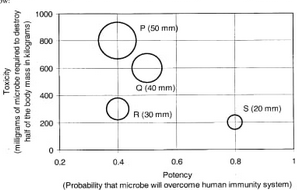
\includegraphics[width=0.5\linewidth]{figs/fig5.png}
    \caption{}
    \label{fig5}
\end{figure}


A pharmaceutical company is contemplating the development of a vaccine against the most dangerous microbe. Which microbe should the company target in its first attempt?  
\begin{enumerate}
\begin{multicols}{4}
    \item P
    \item Q
    \item R
    \item S
    \end{multicols}
\end{enumerate}

\item  \textbf{Few school curricula include a unit on how to deal with bereavement and grief, and yet all students at some point in their lives suffer from losses through death and parting.} 

Based on the above passage, which topic would not be included in a unit on bereavement?  \hfill \textbf{(GATE EE 2025)}
\begin{enumerate}
    \item how to write a letter of condolence
    \item what emotional stages are passed through in the healing process
    \item what the leading causes of death are
    \item how to give support to a grieving friend
\end{enumerate}
\begin{center}
    \textbf{END OF THE QUESTION PAPER}
\end{center}






\end{enumerate}
\end{document}
